\documentclass{article}
\usepackage{graphicx} % Required for inserting images
\usepackage{authblk}
\usepackage{amsmath}
\usepackage{amsfonts}
\usepackage{xcolor}
\usepackage{dsfont}
\usepackage{placeins} % \FloatBarrier keeps figures within their (sub)section
% Let figures share pages with text (avoids half-empty pages)
\renewcommand{\topfraction}{0.9}
\renewcommand{\bottomfraction}{0.8}
\renewcommand{\textfraction}{0.07}
\renewcommand{\floatpagefraction}{0.8}
\setcounter{topnumber}{3}
\setcounter{bottomnumber}{2}
\setcounter{totalnumber}{4}

\title{Using surrogate indices to improve high-dimensional trial-level surrogates of inactivated influenza vaccination immunogenicity}
\author[]{Florian Stijven, Arthur Hughes}
\date{}

\begin{document}

\maketitle

\section*{Proposal abstract}

Modern vaccine studies often measure high-dimensional biomarkers, like transcriptomics, alongside clinically relevant immune response measures, such as antibody responses. These complex markers may be good surrogate candidates, but their high-dimensionality and complexity represent significant challenges for surrogate evaluation. 

The RISE-Meta framework is an example of a robust method for high-dimensional surrogate screening and evaluation in the multi-study setting, but is limited in multiple ways. Namely, RISE-Meta 1) does not take into account the contribution of baseline covariates; and 2) does not consider biologically informed groups of candidate predictors.

The surrogate index (SI) represents a natural way to address these two limitations. The surrogate index is a transformation of surrogate candidate(s) and baseline covariates learned as a prediction of the primary endpoint value. This represents a principled way to combine complex information on multiple surrogate candidates and covariates which, under certain conditions, provides an optimal transformation in terms of trial-level surrogacy. The SI framework was extended to the meta-analytic setting in Stijven and Gilbert (2025), allowing the inclusion of data from multiple trials, to assess the trial-level surrogacy of a SI-transformed candidate surrogate.

In this article, we apply the SI framework combined with RISE-Meta to multi-study inactivated influenza vaccine data to evaluate transcriptomic markers as candidate surrogates of vaccine immunogenicity. In particular, in the first stage, we use the SI to construct, for each of a number of \textit{gene sets} (biologically related groups of genes), a univariate summary of the gene expression profile, taking into account baseline covariate information. The same summary is applied to the pre- and post-vaccination expression of each individual, so that the paired structure of the data is preserved. Then we use these paired surrogate indices as inputs to RISE-Meta for a robust evaluation of the trial-level surrogacy of each gene set-level summary. 

\subsection*{Data Structure and Notation}

Consider data from $K$ studies, indexed $k = 1, \dots, K$, with individuals $i = 1, \dots, n_k$ within study $k$.

\paragraph{Study design.} Each study is a single-arm, pre-post study of one TIV formulation: the same individuals are measured before and after vaccination, and there is no concurrent control arm. The effect of vaccination is quantified by comparing each individual's post-vaccination measurement with their own pre-vaccination measurement (a paired design).

\paragraph{Clinical endpoint.} Each study's TIV formulation targets three influenza strains, $\ell = 1, 2, 3$, corresponding to one A/H1N1, one A/H3N2, and one B strain. The response is measured at two time points, pre- and post-vaccination, common across studies, $t \in \{0,1\}$. Let $Y_{kit\ell}$ denote the (log) HAI titer for individual $i$ in study $k$ against strain $\ell$ at time $t \in \{0,1\}$, and let
\[
\boldsymbol{Y}_{kit} = (Y_{kit1}, Y_{kit2}, Y_{kit3})
\]
denote the vector of strain-specific antibody responses at time $t$.

\textcolor{blue}{Arthur: the three-strain outcome can be handled in two ways: (i) summarise $\boldsymbol{Y}_{ki}$ into a scalar response or (ii) analyse each strain $\ell$ separately, giving strain-specific SIs and surrogacy assessments, which also allows comparing surrogate quality across strains.}

\paragraph{Surrogate candidates.} Gene expression is measured before vaccination and at a single post-vaccination time point $t_S$ that is common across all studies. Let $\boldsymbol{S}_{kit} \in \mathbb{R}^p$ denote the vector of $p$ gene expression features for individual $i$ in study $k$ at time $t \in \{0,1\}$, where $t=0$ is pre-vaccination and $t=1$ corresponds to $t_S$ post-vaccination. Note that ``post-vaccination'' refers to different times for the surrogate ($t_S$) and for the clinical endpoint. Features are grouped into $G$ pre-specified and non-distinct gene sets $\mathcal{G}_1, \dots, \mathcal{G}_G \subseteq \{1, \dots, p\}$, and we write $\boldsymbol{S}_{kit}^{(g)} = (S_{kitj})_{j \in \mathcal{G}_g}$ for the sub-vector of features in gene set $g$.

\textcolor{blue}{Arthur: restricting to a single common time point means that the full longitudinal profile is not used. Perhaps we could consider multiple post-vaccination time points later, though these would have to be common across studies. We would have to consider the balance of complexity and information gain by including more time points.}

\paragraph{Baseline covariates.} Let $X_{ki} \in \mathbb{R}^q$ denote individual-level baseline covariates (e.g.\ age, sex), and $W_k \in \mathbb{R}^r$ trial-level covariates (e.g.\ season).

\textcolor{red}{Florian: It may be better to drop trial-level covariates. A main concern with the surrogate-index approach is trial-level overfitting. If we have trial-level covariates (or individual-level covariates that are proxies for trial-level covariates), this could lead to practical problems. }

\textcolor{blue}{I am OK with this, I don't believe we will have many trial-level covariates which are shared across trials in any case.}

\paragraph{Observed data.} For each individual,
\[
\mathcal{D}_{ki} = \big\{ (\boldsymbol{S}_{ki0}, \boldsymbol{S}_{ki1}),\ (\boldsymbol{Y}_{ki0}, \boldsymbol{Y}_{ki1}),\ X_{ki} \big\},\qquad k = 1,\dots,K,\ i = 1,\dots,n_k,
\]
(with trial-level covariates $\{W_k\}_{k=1}^K$ if desired).

\paragraph{Surrogate index.} Let $\tilde{Y}_{kit}$ denote the scalar endpoint under analysis: either $Y_{kit\ell}$ for a fixed strain $\ell$, or a summary of $\boldsymbol{Y}_{kit}$ computed separately at each time $t$. For gene set $g$, the surrogate index is
\[
\mathrm{SI}^{(g)}_{kit} = f_g\big(\boldsymbol{S}_{kit}^{(g)}, X_{ki}\big), \qquad f_g(\boldsymbol{s}, x) = E\big[\tilde{Y}_{kit} \mid \boldsymbol{S}_{kit}^{(g)} = \boldsymbol{s},\ X_{ki} = x\big],
\]
where the expectation is taken over studies and over both time points. The function $f_g$ does not depend on $t$ (or on $k$): the same function is applied to the pre- and post-vaccination expression, so that the change $\mathrm{SI}^{(g)}_{ki1} - \mathrm{SI}^{(g)}_{ki0}$ reflects only changes in gene expression. The transformation thus yields a pre-post pair $(\mathrm{SI}^{(g)}_{ki0}, \mathrm{SI}^{(g)}_{ki1})$ for each individual, which is analysed alongside $(\tilde{Y}_{ki0}, \tilde{Y}_{ki1})$.

\subsection*{Data-Generating Mechanism}


\textcolor{red}{Florian: I like to be very explicit about the data-generating mechanism and the target parameter and possible identifying (untestable) assumptions. Ideally, we would not make any testable assumptions.}

Each study $k$ has its own distribution $P_k$ of the individual-level data, and $P_1, \dots, P_K$ are independent draws from a population of studies $\mathcal{P}$. Given $P_k$, the observations in study $k$ are i.i.d.:
\[
O_{ki} = \big\{ (\boldsymbol{S}_{ki0}, \boldsymbol{S}_{ki1}),\ (\boldsymbol{Y}_{ki0}, \boldsymbol{Y}_{ki1}),\ X_{ki} \big\} \mid P_k \sim P_k, \qquad i = 1, \dots, n_k.
\]
Every individual is vaccinated at $t=0$ and measured at both $t= 0$ and $t=1$. Let $(\boldsymbol{S}^{0}_{ki}, \boldsymbol{Y}^{0}_{ki})$ and $(\boldsymbol{S}^{1}_{ki}, \boldsymbol{Y}^{1}_{ki})$ denote the potential values at the post-vaccination time without and with vaccination, with $X_{ki}$ unaffected by vaccination. No parametric model is assumed for $P_k$ or $\mathcal{P}$.

\subsection*{Target Parameters}

The estimand follows RISE-Meta in the paired case. Let $G(a,b) = \mathds{1}(a > b) + \tfrac12 \mathds{1}(a = b)$, and assume without loss of generality that larger values of $\tilde{Y}$ and of the SI are better.

\paragraph{Within-study parameter.} For gene set $g$ and study $k$, let
\[
U_{Y,k} = E_k\big[ G(\tilde{Y}_{ki1}, \tilde{Y}_{ki0}) \big], \qquad
U_{g,k} = E_k\big[ G(\mathrm{SI}^{(g)}_{ki1}, \mathrm{SI}^{(g)}_{ki0}) \big], \qquad
\delta_{g,k} = U_{Y,k} - U_{g,k},
\]
where $E_k$ is the expectation over individuals in study $k$. $U_{Y,k}$ and $U_{g,k}$ are the probabilities that an individual's post-vaccination value exceeds their own pre-vaccination value, for the endpoint and the SI respectively. The parameter $\delta_{g,k}$ is the bias in estimating the effect on the endpoint from the SI alone; the closer to $0$, the better the surrogate.

\paragraph{Trial-level parameter.} Across studies, $\delta_{g,k} \sim N(\mu_g, \tau_g^2)$, where $\mu_g$ is the mean and $\tau_g^2$ the between-study variance. The classical target parameter is $\mu_g$, with $\tau_g^2$ describing heterogeneity across studies. Gene set $g$ is a trial-level surrogate if
\[
H_0: \mu_g \notin (-\varepsilon, \varepsilon) \quad \text{versus} \quad H_1: \mu_g \in (-\varepsilon, \varepsilon),
\]
for a pre-specified equivalence margin $\varepsilon$. These parameters are defined for each gene set $g$.

Instead of the mean of the distribution of the within-study parameters, we may be interested in the distribution of the within-study parameter in a new trial. This addresses the fact that, when between-study heterogeneity is high, the mean within-study parameter may be precise and close to 0, but this does not imply that an observation from a new trial is expected to be close to 0 (i.e. an unreliable surrogate).

\textcolor{red}{Arthur: this predictive interval based test is not described in the first version of RISE-Meta, but is described in my thesis and in the current version of RISE-Meta, which is being revised.}

\subsection*{Causal Interpretation and Assumptions}

Since these data are not typically from RCTs with a control group, we use pre-post data to describe changes attributable to vaccination. Therefore, typically these measures may be interpreted in terms of statistical association. However, under certain untestable assumptions, this can have a causal interpretation:

\begin{enumerate}
    \item \textbf{Stable unit treatment value assumption.} Within each study, the observed post-vaccination values equal $Y^{1}_{ki}$ and $\mathrm{SI}^{1}_{ki}$, there is a single version of treatment, and there is no interference between individuals.
    \textcolor{blue}{Arthur: consistency seems reasonable. Perhaps no interference would be relevant in certain trial designs in the data (e.g. there is one which only vaccinates NIH employees, and flu may be spread in work environments). Single version of treatment seems OK, since we only need this to hold within each study, but formulations are allowed to differ across studies.}
    \item \textbf{No time effect.} Without vaccination, an individual's pre-vaccination values would be unchanged at the post-vaccination time: $\tilde{Y}_{ki0} = Y^{0}_{ki}$ and $\mathrm{SI}^{(g)}_{ki0} = \mathrm{SI}^{0}_{ki}$.
    \textcolor{blue}{Arthur: I think the longer term time-based effects, like seasonality, natural infection, waning immunity etc. would not be problems due to the short time scales in the study designs (up to 4 weeks for the antibodies). As for shorter term effects, like circadian rhythm, stress, diet, etc, these can have an impact on gene expression regardless of vaccination. I suppose that if we assume that the sampling time during the day is pretty much random and not systematically different between time 0 and time 1, this is ok, since this is just a source of noise which will be smoothed out. Perhaps an argument could be made that the immune genes we are interested in are less likely to be affected by these short term factors.}
    \item \textbf{No selection on baseline values.} Enrolment does not depend on pre-vaccination values (no regression to the mean), and loss to follow-up between visits is ignorable. \textcolor{blue}{Arthur: think this is reasonable.}
    \item \textbf{Comparable measurements.} Within each study, pre- and post-vaccination samples are measured and processed comparably.
    \textcolor{blue}{Arthur: think this is reasonable since each study will have the same investigators, and the data has been normalised for batch effects. The within-study parameters are rank-based, so they are invariant to monotone differences in scale between studies.}
    \item \textbf{No surrogate paradox.} For all $s, y$, writing $\mathrm{SI}$ for $\mathrm{SI}^{(g)}$: (C1) $P(Y^{a} > y \mid \mathrm{SI}^{a} = s)$ is increasing in $s$; (C2) $P(\mathrm{SI}^{1} > s) \ge P(\mathrm{SI}^{0} > s)$; (C3) $P(Y^{1} > y \mid \mathrm{SI}^{1} = s) \ge P(Y^{0} > y \mid \mathrm{SI}^{0} = s)$.
    \textcolor{blue}{Arthur: these are the untestable assumptions to avoid the surrogate paradox we state in RISE. They are needed to interpret surrogacy, not to identify $U_{Y,k}$ and $U_{g,k}$ causally.}
    \item \textbf{Exchangeable studies.} Studies are independent draws from a population of studies, with individuals i.i.d.\ within each study.
    \textcolor{blue}{Arthur: these are classic and I have no reason to doubt them in this case. Perhaps the fact that some of the same investigators are involved across multiple studies is problematic, but unlikely too much.}
\end{enumerate}

\section*{Application}

\paragraph{Questions.}
\begin{enumerate}
    \item Are gene set-level surrogate indices of early post-vaccination gene expression trial-level surrogates for the HAI antibody response to inactivated influenza vaccination?
    \item Does the SI provide stronger surrogates than considering each gene individually? Are SI surrogates stronger than simple gene set summaries (e.g. mean expression in set)?
    \item Are there particular methods for estimating the SI which produce better surrogates (e.g. glm, lasso, elastic net, random forest, XGboost, super learner)?
    \item Which biological functions produce the best surrogates? Which are the individual genes/covariates which most contribute to such surrogacy?
    \item Does the quality of the surrogate differ between the three influenza strains?
\end{enumerate}

\paragraph{Rationale.} Gene expression is available within days of vaccination, whereas the antibody response is measured around 28 days after vaccination, so a valid surrogate would allow earlier screening of vaccine candidates. It also helps to understand which biological processes are associated with the antibody response at the trial-level.

\textcolor{blue}{Arthur: perhaps the second point on vaccine-level inference is more relevant, unless we can find a very strong and reliable surrogate.}

\paragraph{Data.} Studies from the Immune Signatures 2 dataset. Healthy adults receiving TIV with gene expression and antibodies against the 3 vaccine strains measured before and after vaccination (day 0 and day 1, 3 or 7 for gene expression; day 0 and day 28 for antibodies). Baseline covariates: age, sex, perhaps race. Gene sets: Blood Transcriptional Modules (BTMs). See the Data description section for the studies and endpoint used.

\paragraph{Analysis.} In the first stage, we construct the SI for each gene set (and each strain, or the scalar summary). In the second stage, we apply RISE-Meta to the paired SI and endpoint, with a pre-specified equivalence margin $\varepsilon$, and control the false discovery rate across gene sets and strains.\textcolor{blue}{Arthur: we should discuss cross-fitting and how this should be used to avoid double-dipping/overfitting.}

\paragraph{Limitations.}
\begin{itemize}
    \item The antibody markers are defined slightly differently across studies
    \textcolor{blue}{Arthur: as we discussed, I think we can make the assumption that, since the vaccines are matched to their strains, that this will be unlikely to pose a problem.}
    \item A single time point used (although no reason why we can't use multiple common time points, but we are just limited by number of studies)
    \item Few studies (day 1: 5, day 3: 8, day 7: 13; Figure~\ref{fig:analysable})
    \item The pre-post design means a causal interpretation relies on the untestable assumptions above.
\end{itemize}

\section*{Data description}

This section describes the inactivated influenza vaccine studies in the Immune Signatures 2 (IS2) dataset. Figure~\ref{fig:analysable} shows, for three post-vaccination time points (days 1, 3 and 7), the number of individuals with complete paired data: gene expression at baseline and at the given day, and antibody titres (HAI, or neutralising antibodies when HAI is unavailable) against each of the three vaccine strains at baseline and day 28. Participants from the type 2 diabetes cohorts of SDY1119 were removed, as were studies with fewer than 5 complete individuals.

Figure~\ref{fig:uy} shows the within-study effect of vaccination on the endpoint on the probability scale, $U_{Y,k}$. Here, $\tilde{Y}$ is the mean of the log$_2$ titres against the three vaccine strains.

\begin{figure}[htbp]
    \centering
    \makebox[\textwidth][c]{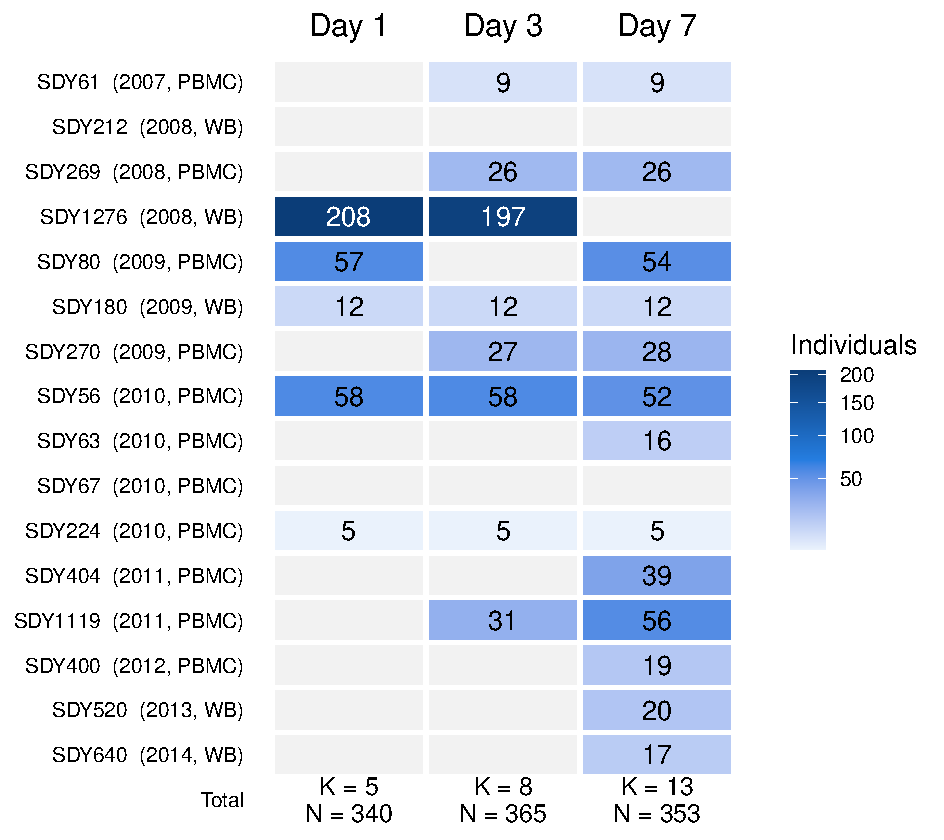
\includegraphics{figures/analysable_by_day_hai_nab_3subtypes.pdf}}
    \caption{Number of individuals with complete paired data, by study (season, cell type) and post-vaccination gene expression day. WB: whole blood.}
    \label{fig:analysable}
\end{figure}

\begin{figure}[htbp]
    \centering
    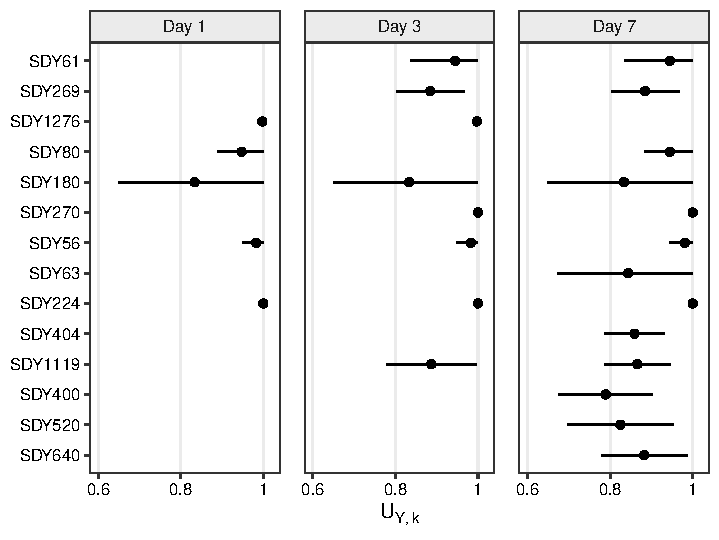
\includegraphics[width=\textwidth]{figures/endpoint_uy_by_study.pdf}
    \caption{Within-study effect of vaccination on the antibody endpoint, $U_{Y,k}$, with 95\% confidence intervals, by study and post-vaccination gene expression day.}
    \label{fig:uy}
\end{figure}

\FloatBarrier
\section*{Application to all gene sets at day 7}

Here, I use ridge regression to learn surrogate indices through cross-fitting for each gene-set at day 7 post-vaccination. 
\begin{itemize}
    \item \textbf{Data.} The 13 studies available at day 7 (Figure~\ref{fig:analysable}). Genes and $\tilde{Y}$ are centred and scaled within study, pooling both time points; this removes platform and assay differences between studies without changing anyone's direction of change.
    \item \textbf{Gene sets.} Blood transcriptional modules (BTMs) with at least 5 genes measured in every study, excluding unannotated modules.
    \item \textbf{Surrogate index.} $f_g$ is learned with ridge regression on both time points pooled, and the same $f_g$ is applied to the pre- and post-vaccination expression of each individual. To avoid overfitting at the trial level, $f_g$ is cross-fitted leave-one-study-out: the SI of study $k$ is computed with a function learned on the other studies only.
    \item \textbf{Evaluation.} Each candidate surrogate is evaluated with paired RISE-Meta, with equivalence margin $\varepsilon = 0.2$, testing whether the prediction interval of $\delta$ lies within the margin.
    \item \textbf{Figures.} Pooled $\delta$ is shown with its 90\% confidence interval (thick) and 90\% prediction interval (thin); the shaded band is the equivalence margin. A candidate is a good trial-level surrogate when its prediction interval lies within the band.
\end{itemize}

\subsection*{Screening of all gene sets}

The SI of each gene set is evaluated with RISE-Meta, with Benjamini--Hochberg correction across gene sets; studies with a zero within-study standard error are removed for the affected gene set only. After correction, no gene set passes the test. Figure~\ref{fig:screen_si_screen} shows the screening results for the top 20 gene sets. The top gene set is M156.0 (plasma cells \& B cells, immunoglobulins), which is studied in more detail in the next section.

\begin{figure}[htbp]
    \centering
    \makebox[\textwidth][c]{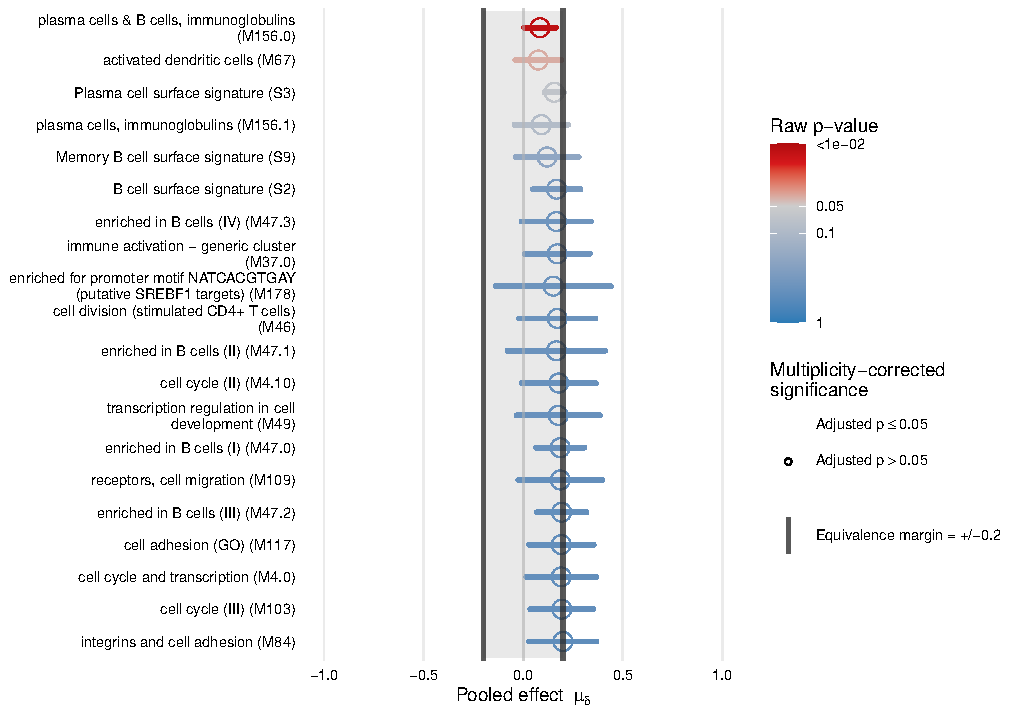
\includegraphics[width = 15cm]{figures/screen_si_screen.pdf}}
    \caption{RISE-Meta screening results for the SI (ridge): top 20 gene sets by p-value, day 7. Pooled $\delta$ with 90\% prediction interval. Shaded: equivalence margin.}
    \label{fig:screen_si_screen}
\end{figure}

\FloatBarrier
\subsection*{Mean versus surrogate index}

I evaluated whether the SI improved on a simple summary of within-geneset expression (mean) across genesets (Figure~\ref{fig:screen_mean_vs_si}).  

\begin{figure}[htbp]
    \centering
    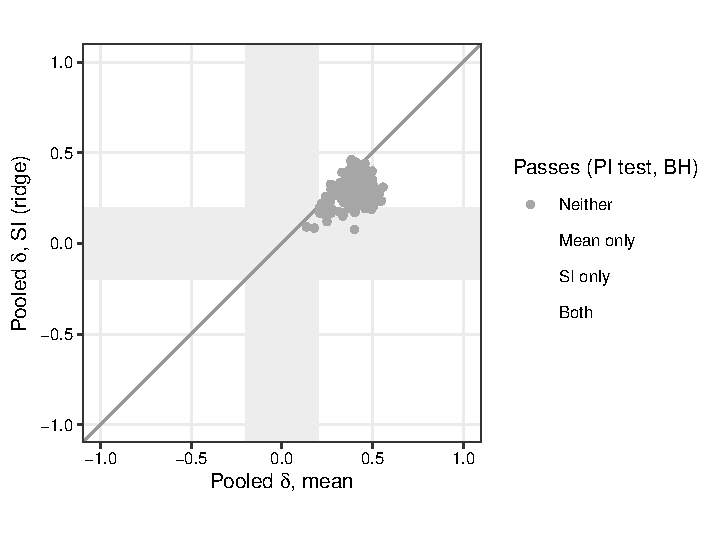
\includegraphics[width=\textwidth]{figures/screen_mean_vs_si.pdf}
    \caption{Pooled $\delta$ of the mean and of the SI (ridge), one point per gene set, day 7. The shaded region denotes the limits for the equivalence test ($\epsilon = 0.2$).}
    \label{fig:screen_mean_vs_si}
\end{figure}

\FloatBarrier
\section*{Top gene set: M156.0}

Since no genesets pass the equivalence test after multiplicity correction, we can go further simply by examining the top geneset, M156.0 (plasma cells \& B cells, immunoglobulins).

\subsection*{RISE-Meta results for the surrogate index}

Figures~\ref{fig:screen_si_fit} and~\ref{fig:screen_si_forest} show the RISE-Meta fit and forest plots of the SI of M156.0, computed on the same data as the screening.

\begin{figure}[htbp]
    \centering
    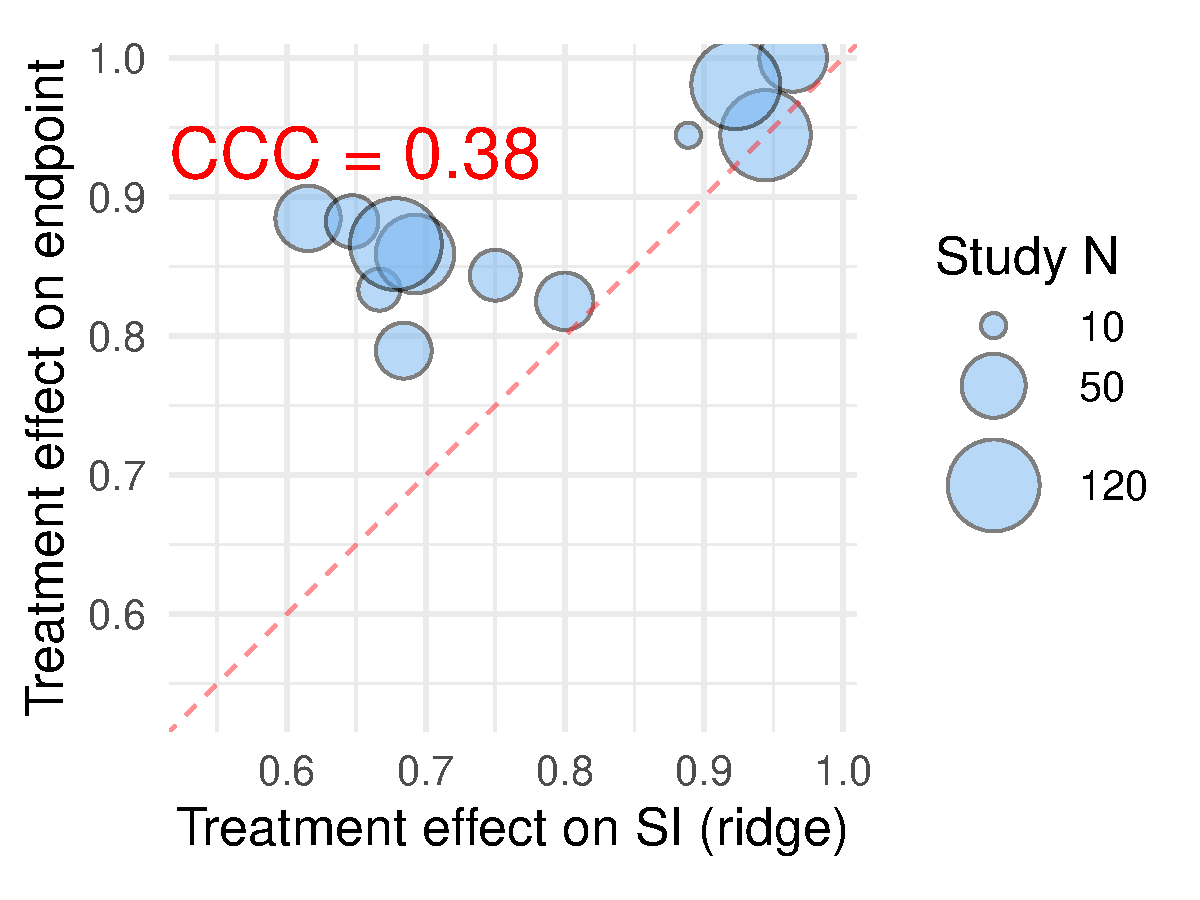
\includegraphics[width=0.75\textwidth]{figures/screen_si_fit.pdf}
    \caption{Plot showing the within-study treatment effect on the clinical endpoint ($U_{Y,k}$) against that on the SI ($U_{S,k}$), one point per study. The CCC is the concordance correlation coefficient.}
    \label{fig:screen_si_fit}
\end{figure}

\begin{figure}[htbp]
    \centering
    \makebox[\textwidth][c]{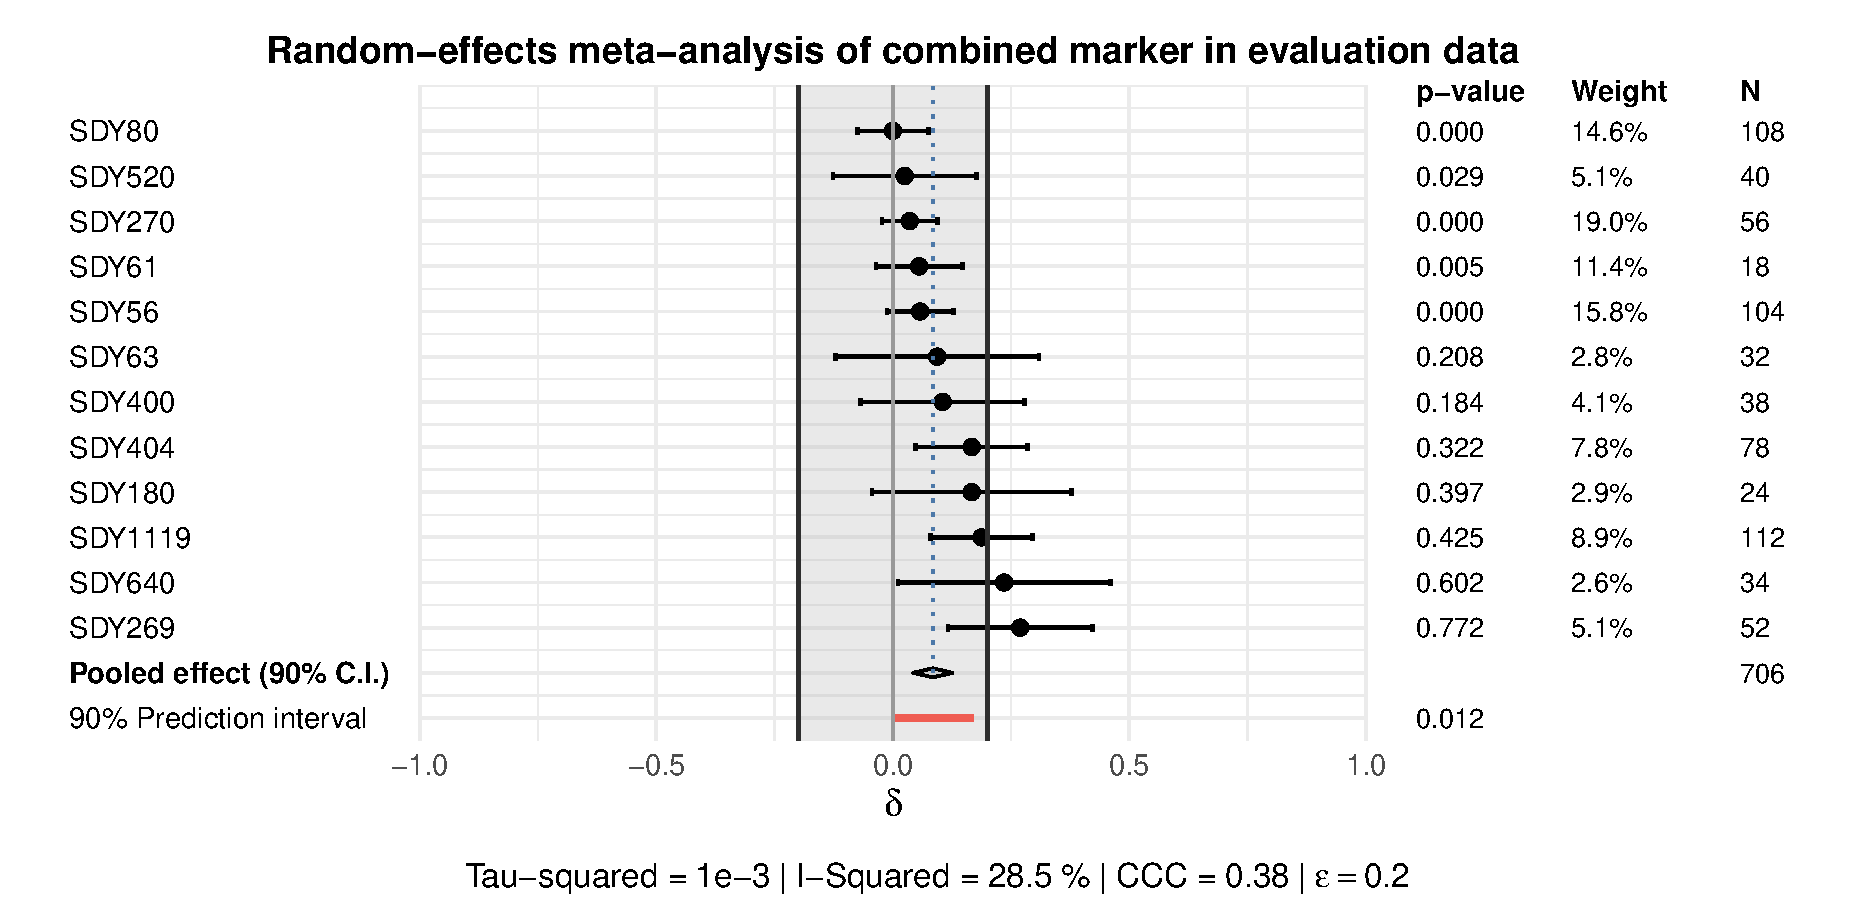
\includegraphics[width=6.3in]{figures/screen_si_forest.pdf}}
    \caption{Forest plot for the SI (ridge) of M156.0 at day 7, computed on the same data as the screening.}
    \label{fig:screen_si_forest}
\end{figure}

\FloatBarrier
\subsection*{Is the SI better than simple aggregation?}

Here, I compare the SI with three simple aggregations of genes in the set (mean, median, max). 

\begin{figure}[htbp]
    \centering
    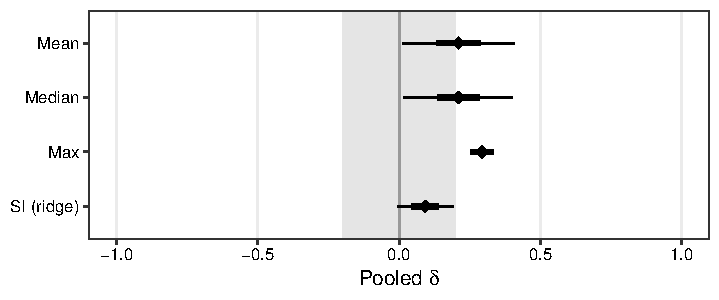
\includegraphics[width=\textwidth]{figures/example_geneset_aggregation_pooled.pdf}
    \caption{Pooled $\delta$ for three simple aggregations of M156.0 at day 7 and the SI (ridge regression).}
    \label{fig:example_agg_pooled}
\end{figure}

\FloatBarrier
\subsection*{Is the geneset SI better than the individual genes in the set?}

Here, I compare the SI with each gene of the set on its own. Genes are re-oriented such that larger values are better, using the sign of its correlation with $Y$ within other studies. 

\begin{figure}[htbp]
    \centering
    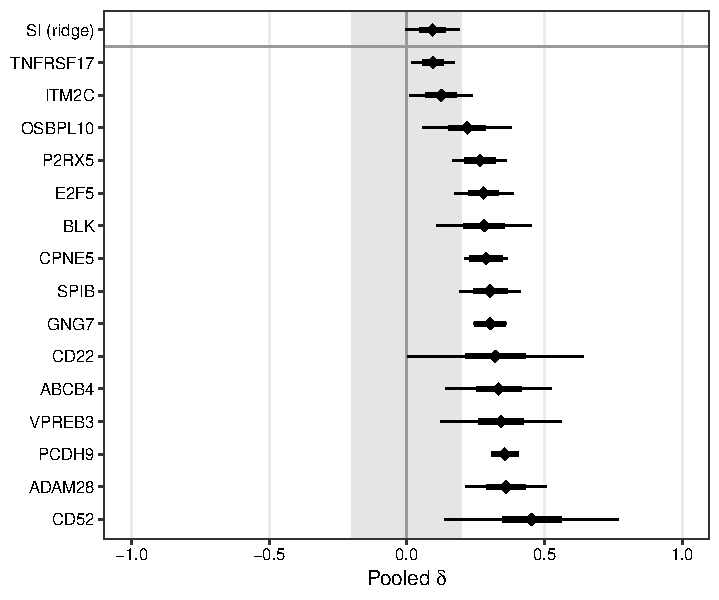
\includegraphics[width=0.85\textwidth]{figures/example_geneset_single_genes.pdf}
    \caption{Pooled $\delta$ for the SI (ridge, top) and each gene of M156.0.}
    \label{fig:example_genes}
\end{figure}

\FloatBarrier
\subsection*{Impact of the SI learner}

I compare different methods for learning the SI (ridge, lasso and elastic net regression, unpenalised linear regression, partial least squares (PLS), sparse PLS, random forest, XGBoost, and a super learner combining all of these except XGBoost). 

\begin{figure}[htbp]
    \centering
    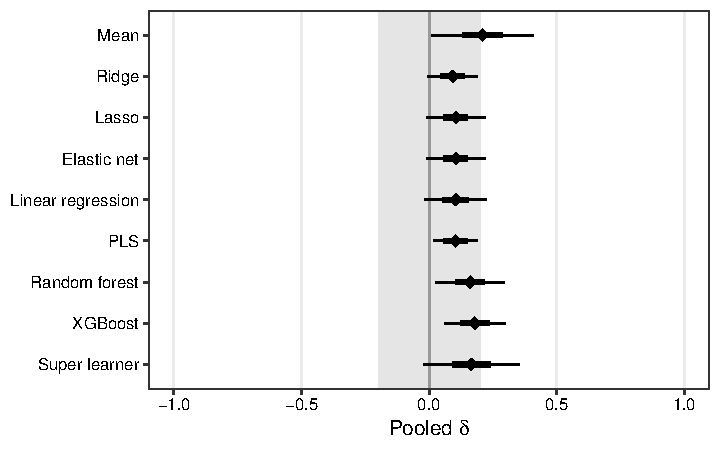
\includegraphics[width=\textwidth]{figures/example_geneset_learners.pdf}
    \caption{Pooled $\delta$ for the mean expression of M156.0 and the SI learned with each method.}
    \label{fig:example_learners}
\end{figure}

\FloatBarrier
\subsection*{Impact of baseline covariates}

I examine the impact of baseline covariates (age and sex) in the SI. 
\begin{figure}[htbp]
    \centering
    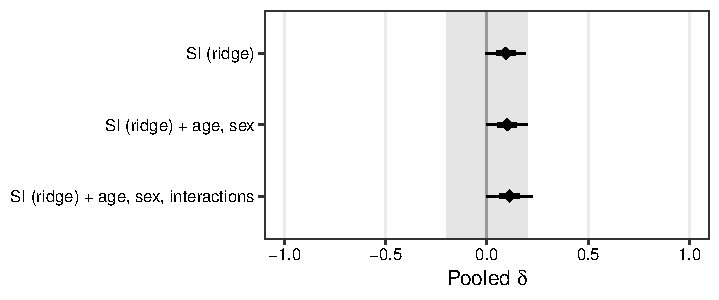
\includegraphics[width=\textwidth]{figures/example_geneset_covariates.pdf}
    \caption{Pooled $\delta$ for the SI (ridge) of M156.0 without covariates, with age and sex, and with age, sex and gene $\times$ covariate interactions.}
    \label{fig:example_covariates}
\end{figure}

\FloatBarrier
\subsection*{Interpreting the surrogate index}

The SI can be interpreted through the coefficients of the ridge regression. Figure~\ref{fig:example_interpretation} shows the coefficients of the ridge SI fitted on all studies, with their range over the leave-one-study-out fits.

\begin{figure}[htbp]
    \centering
    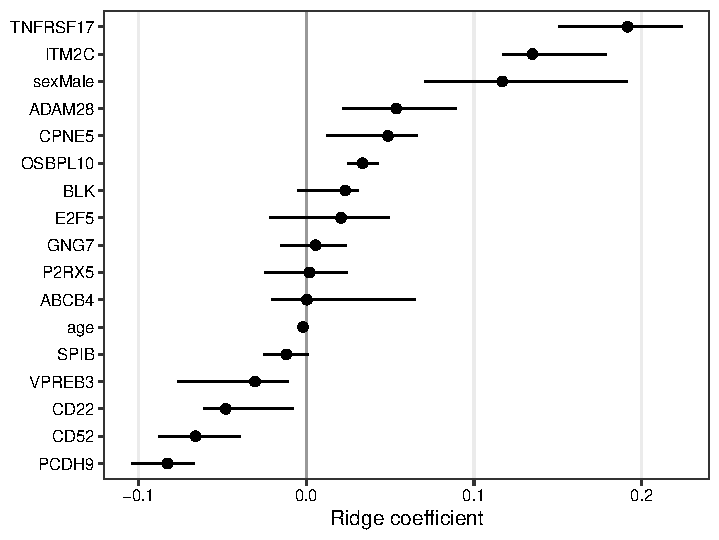
\includegraphics[width=\textwidth]{figures/example_geneset_interpretation.pdf}
    \caption{Ridge SI coefficients of the genes in M156.0 (standardised expression). Point: fit on all studies; bar: range over the leave-one-study-out fits.}
    \label{fig:example_interpretation}
\end{figure}

\FloatBarrier
\subsection*{Individual-level predictions}

Beyond trial-level surrogacy, the SI can be judged on how well it predicts individual antibody responses. Figure~\ref{fig:example_prediction} compares these predictions with the observed responses (centred and scaled within study), at baseline and at day 28, in each held-out study.

\begin{figure}[htbp]
    \centering
    \makebox[\textwidth][c]{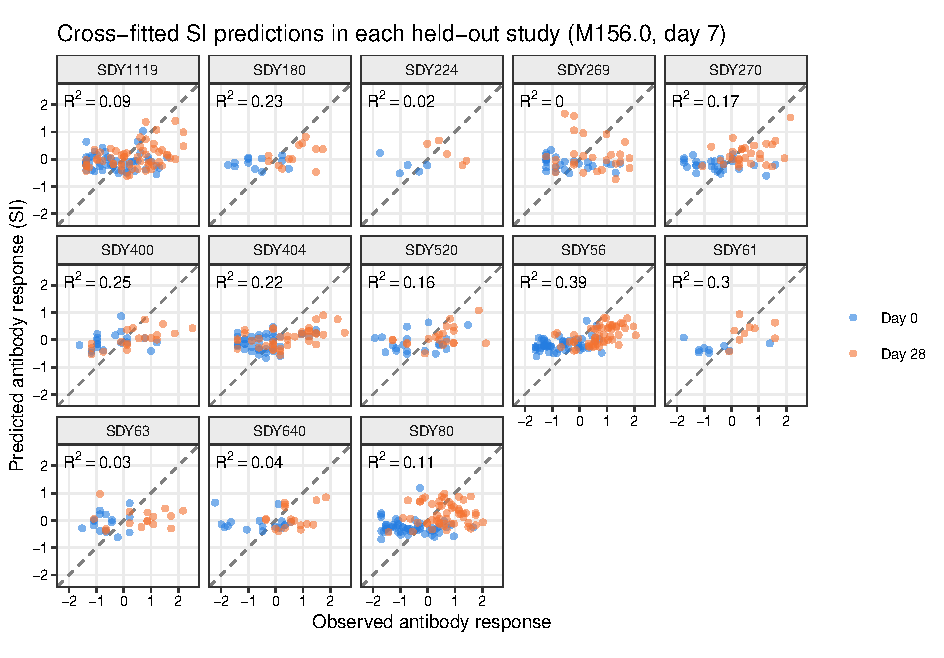
\includegraphics{figures/example_geneset_prediction.pdf}}
    \caption{Predicted (SI, ridge, cross-fitted leave-one-study-out) versus observed antibody response, by held-out study, for M156.0 at day 7. Dashed line: perfect prediction.}
    \label{fig:example_prediction}
\end{figure}

\FloatBarrier
%\subsection*{Without cross-fitting}

%Finally, to see what cross-fitting protects against, I repeat the analysis with an SI fitted once on all studies and applied to the same studies. In this case, the antibody data of each study contribute to the SI on which that study is then evaluated. Figure~\ref{fig:example_nocf_prediction} shows the resulting (in-sample) predictions, to compare with Figure~\ref{fig:example_prediction}, and Figure~\ref{fig:example_nocf_pooled} repeats the comparison of Figure~\ref{fig:example_agg_pooled} with both the cross-fitted SI and the SI without cross-fitting.

%\begin{figure}[htbp]
%    \centering
%    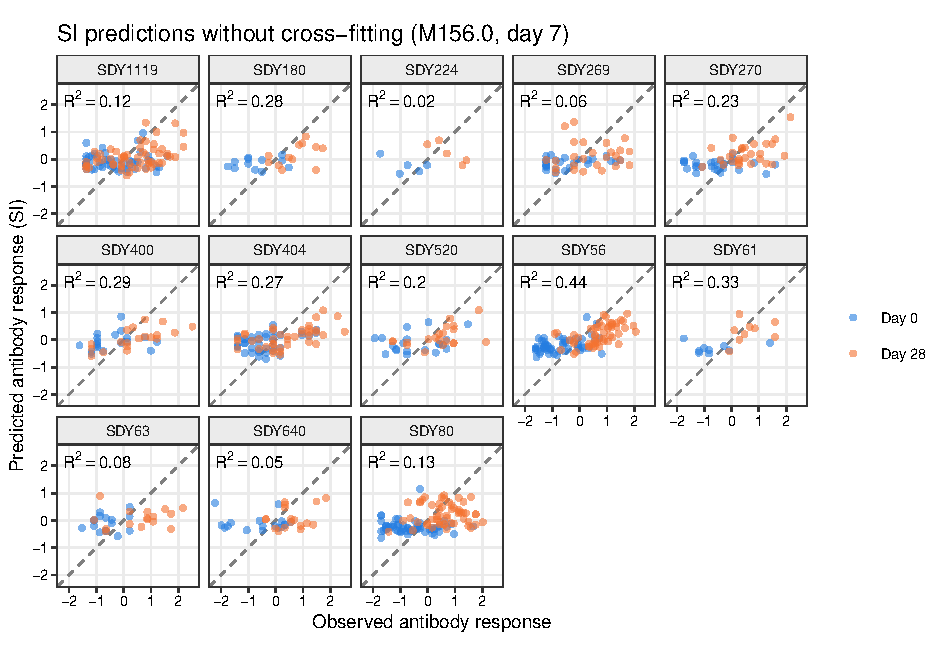
\includegraphics[width=\textwidth]{figures/example_geneset_no_crossfit_prediction.pdf}
%    \caption{Predicted (SI, ridge, fitted on all studies without cross-fitting) versus observed antibody response, by study, for M156.0 at day 7. Dashed line: perfect prediction.}
%    \label{fig:example_nocf_prediction}
%\end{figure}

%\begin{figure}[htbp]
%    \centering
%    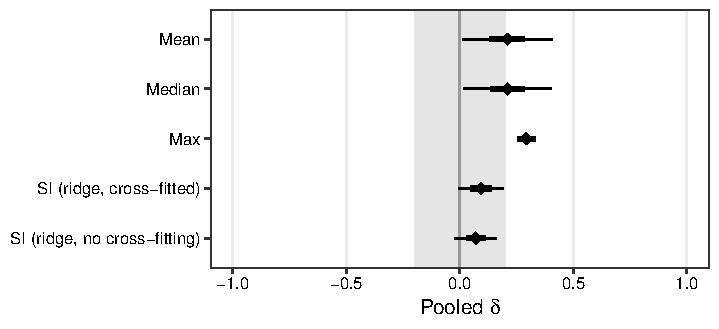
\includegraphics[width=\textwidth]{figures/example_geneset_no_crossfit_pooled.pdf}
%    \caption{Pooled $\delta$ for three simple aggregations of M156.0 and the SI (ridge), with and without cross-fitting.}
%    \label{fig:example_nocf_pooled}
%\end{figure}

\FloatBarrier
%\subsection*{Negative control}

%To check that the SI does not turn any set of genes into a good trial-level surrogate, I repeat this comparison on M1.1 (integrin cell surface interactions (II)), a module chosen at random among those not expected to respond to the vaccine. Figure~\ref{fig:example_negative} compares the pooled estimates.

%\begin{figure}[htbp]
%    \centering
%    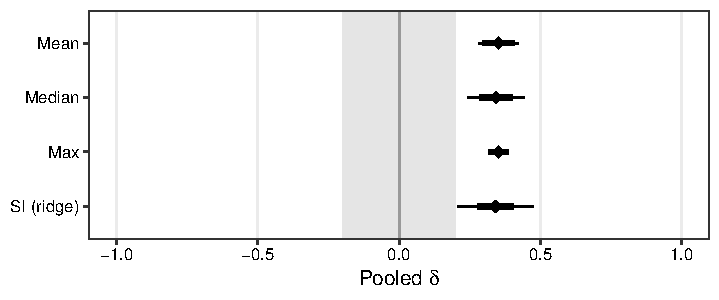
\includegraphics[width=\textwidth]{figures/example_geneset_negative_control.pdf}
%    \caption{Negative control: pooled $\delta$ for three simple aggregations of M1.1 and the SI (ridge).}
%    \label{fig:example_negative}
%\end{figure}

\end{document}
